\section{Spatial proteomics}

\begin{frame}{}
  \begin{center}
    \Large{\textbf{Use case}: spatial proteomics.}
  \end{center}
\end{frame}


\begin{frame}{Cell organisation - regulation of protein localisation}
  \begin{center}
    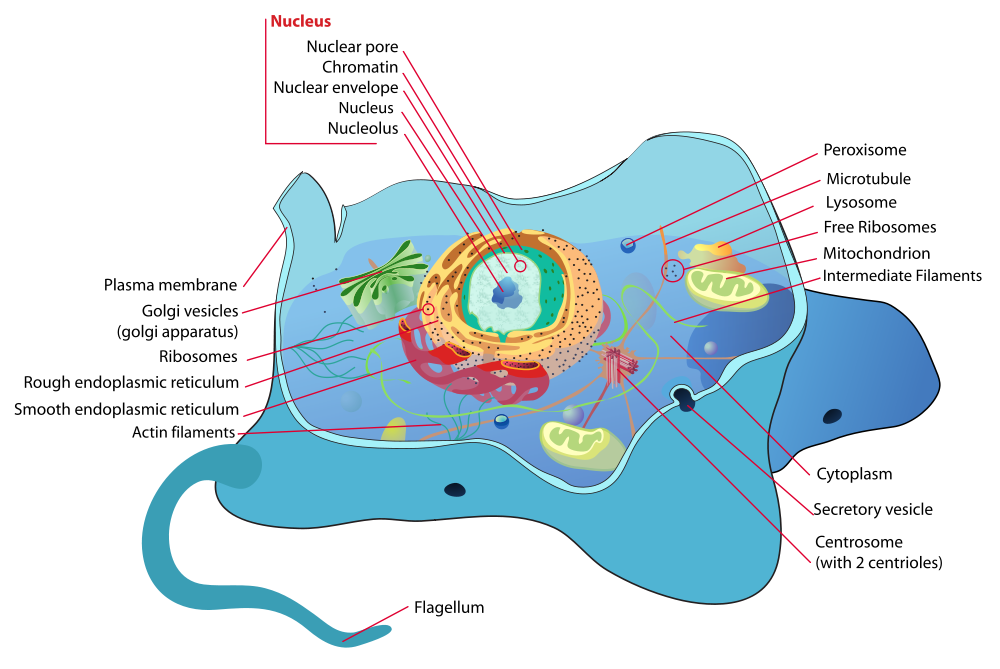
\includegraphics[width=1\linewidth]{figs_all/Animal_cell_structure.png} \\
    \textbf{\textcolor{Blue}{Spatial proteomics}} is the systematic
    study of protein localisations.
  \end{center}

  \tiny Image from Wikipedia
  \url{http://en.wikipedia.org/wiki/Cell_(biology)}.
\end{frame}


\begin{frame}{Spatial proteomics - Why?}

  \begin{itemize}

  \item \textbf{Localisation is function}: Localisation and
    sequestration of proteins within sub-cellular niches is a
    fundamental mechanism for the post-translational regulation of
    protein function.

    \bigskip
      
  \item \textbf{Re-localisation}: \textcolor{Blue}{differentiation}
    stem cells, \textcolor{Blue}{activation} of biological processes.

    \bigskip
    
  \item \textbf{Mis-localisation}: Disruption of the
    targeting/trafficking process alters proper sub-cellular
    localisation, which in turn perturb the cellular functions of the
    proteins.
    
  \end{itemize}
  
\end{frame}



\begin{frame}{Spatial proteomics - How, experimentally}
  \begin{figure}
    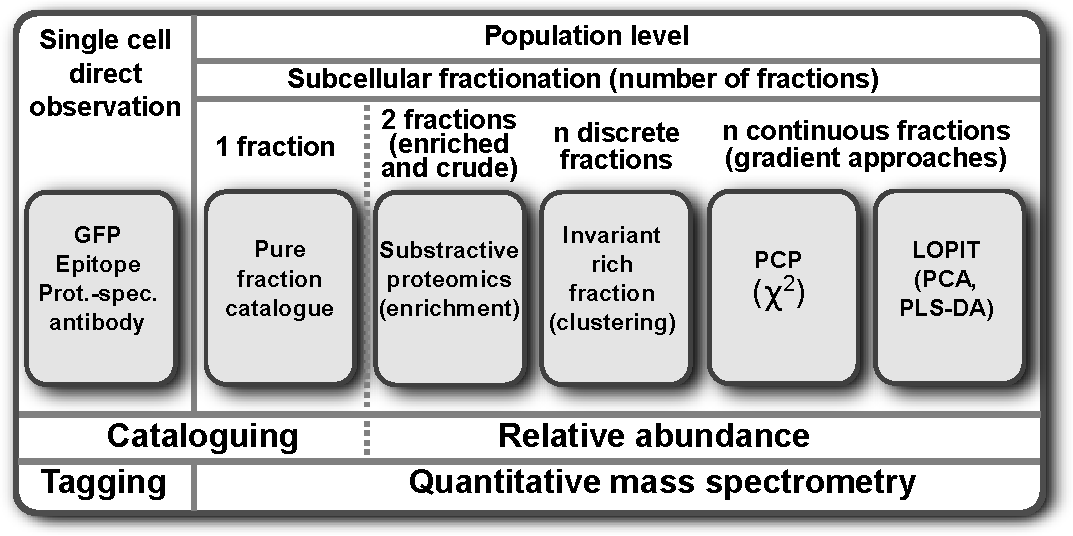
\includegraphics[width=.8\linewidth]{figs_all/F02-expdesigns.pdf}
    \caption{Organelle proteomics approaches
      \citep{Gatto:2010}.}
  \end{figure}

  \textbf{Gradient approaches}: \cite{Dunkley:2006},
  \cite{Foster2006}.

  \bigskip

  \textbf{Explorative/discovery approaches},
  \textcolor{Blue}{steady-state \textbf{global localisation maps}}.
\end{frame}


\begin{frame}{}
  \begin{figure}
    % \includegraphics[width=.8\linewidth]{figs_all/F03-protocols-8plex.pdf}
    % 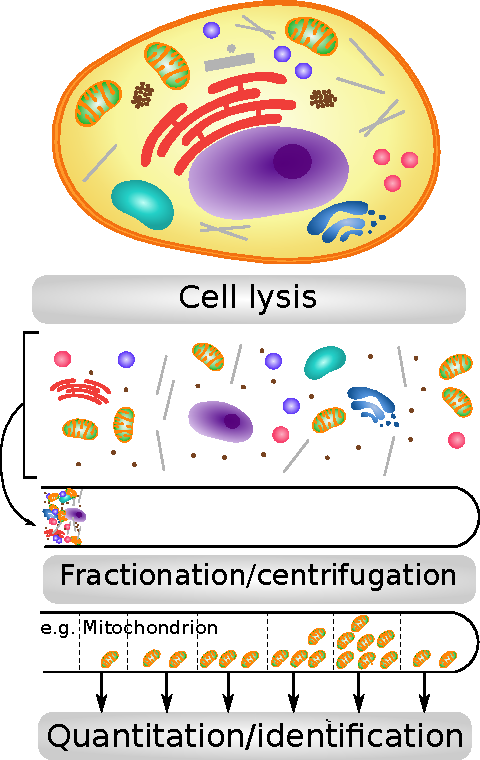
\includegraphics[width=.5\linewidth]{figs_all/expdesign.pdf}
    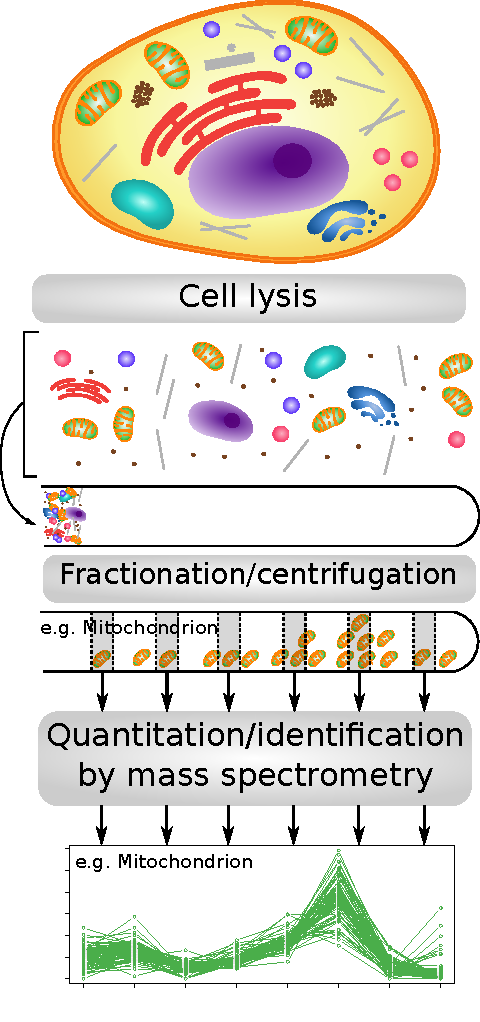
\includegraphics[width=.39\linewidth]{figs_all/workflow_primary.pdf}
  \end{figure}
\end{frame}

\subsubsection*{The data}
\label{sec:data}

\begin{frame}{Quantitation data}
  \begin{center}
    \begin{tabular}{|l|llll|}
      \hline
      & Fraction$_{\text{1}}$ & Fraction$_{\text{2}}$ & \ldots{} & Fraction$_{\text{L}}$ \\
      \hline
      {\bf x}$_{\text{1}}$ & $x_{\text{1,1}}$ & $x_{\text{1,2}}$ & \ldots{} & $x_{\text{1,L}}$ \\
      {\bf x}$_{\text{2}}$ & $x_{\text{2,1}}$ & $x_{\text{2,2}}$ & \ldots{} & $x_{\text{2,L}}$ \\
      {\bf x}$_{\text{3}}$ & $x_{\text{3,1}}$ & $x_{\text{3,2}}$ & \ldots{} & $x_{\text{3,L}}$ \\
      \vdots & \vdots & \vdots & \vdots & \vdots \\
      {\bf x}$_{\text{i}}$ & $x_{\text{i,1}}$ & $x_{\text{i,2}}$ & \ldots{} & $x_{\text{i,L}}$ \\
      \vdots & \vdots & \vdots & \vdots & \vdots \\
      {\bf x}$_{\text{N}}$ & $x_{\text{N,1}}$ & $x_{\text{N,2}}$ & \ldots{} & $x_{\text{N, L}}$ \\
      \hline
    \end{tabular}
  \end{center}
\end{frame}

\begin{frame}{Quantitation data and organelle markers}
  \begin{center}
    \begin{tabular}{|l|llll||l|}
      \hline
      & Fraction$_{\text{1}}$ & Fraction$_{\text{2}}$ & \ldots{} & Fraction$_{\text{L}}$ & markers\\
      \hline
      {\bf x}$_{\text{1}}$ & $x_{\text{1,1}}$ & $x_{\text{1,2}}$ & \ldots{} & $x_{\text{1,L}}$ & unknown \\
      {\bf x}$_{\text{2}}$ & $x_{\text{2,1}}$ & $x_{\text{2,2}}$ & \ldots{} & $x_{\text{2,L}}$ & \textcolor{Red}{$loc_{1}$}\\
      {\bf x}$_{\text{3}}$ & $x_{\text{3,1}}$ & $x_{\text{3,2}}$ & \ldots{} & $x_{\text{3,L}}$ & unknown \\
      \vdots & \vdots & \vdots & \vdots & \vdots & \vdots \\
      {\bf x}$_{\text{i}}$ & $x_{\text{i,1}}$ & $x_{\text{i,2}}$ & \ldots{} & $x_{\text{i,L}}$ & \textcolor{Blue}{$loc_{k}$}\\
      \vdots & \vdots & \vdots & \vdots & \vdots & \vdots\\
      {\bf x}$_{\text{N}}$ & $x_{\text{N,1}}$ & $x_{\text{N,2}}$ & \ldots{} & $x_{\text{N, K}}$ & unknown \\
      \hline
    \end{tabular}
  \end{center}
\end{frame}

\begin{frame}{}
  \begin{center}
    \Large{Data analysis}
  \end{center}
\end{frame}


\subsection*{Data analysis}
\label{sec:comp}

\subsubsection*{Visualisation}
\label{sec:viz}

\begin{frame}{Visualisation}
  \begin{figure}
    \centering
    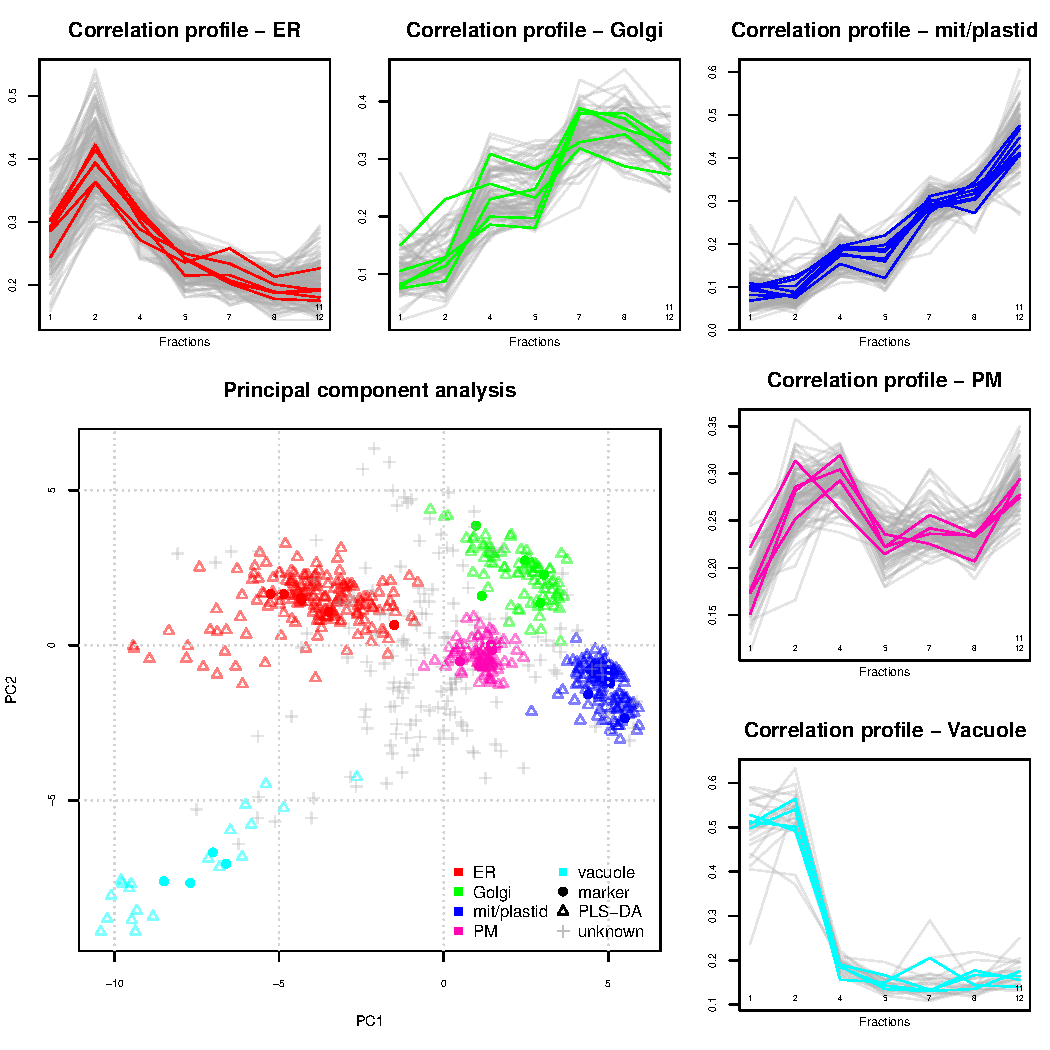
\includegraphics[width=.6\linewidth]{figs_all/F04-analyses.pdf}
    \caption{From \cite{Gatto:2010}, \textit{Arabidopsis thaliana} data
      from \cite{Dunkley:2006}}
  \end{figure}
\end{frame}

\subsubsection*{Machine learning}
\label{sec:ml}

\begin{frame}{Supervised Machine Learning}
  \begin{figure}[h]
    \centering
    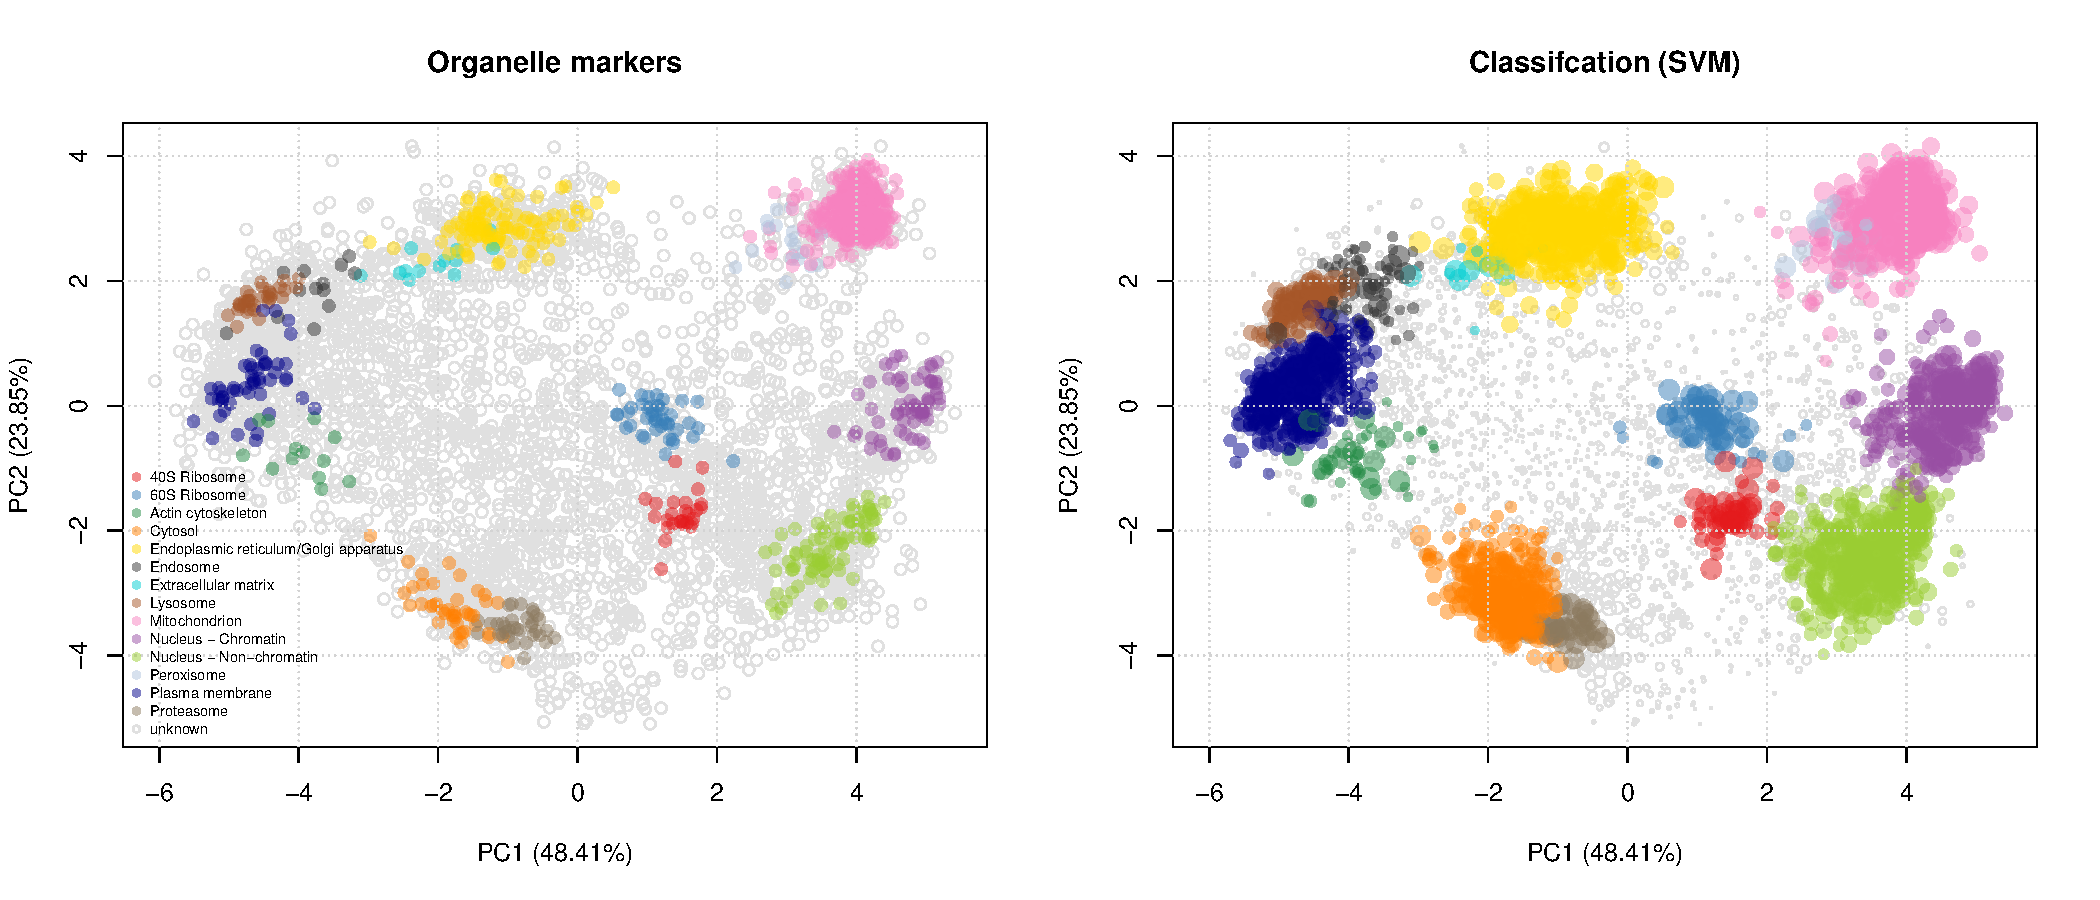
\includegraphics[width=\linewidth]{figs_all/hyperlopit-class.pdf}
    \caption{Support vector machines classifier (after 5\% FDR
      classification cutoff) on the embryonic stem cell data from
      \cite{Christoforou:2016}.}
  \end{figure}
\end{frame}


\subsection{Embracing uncertainty}

\begin{frame}{How much do we learn? How much do we miss?}
  \begin{figure}
    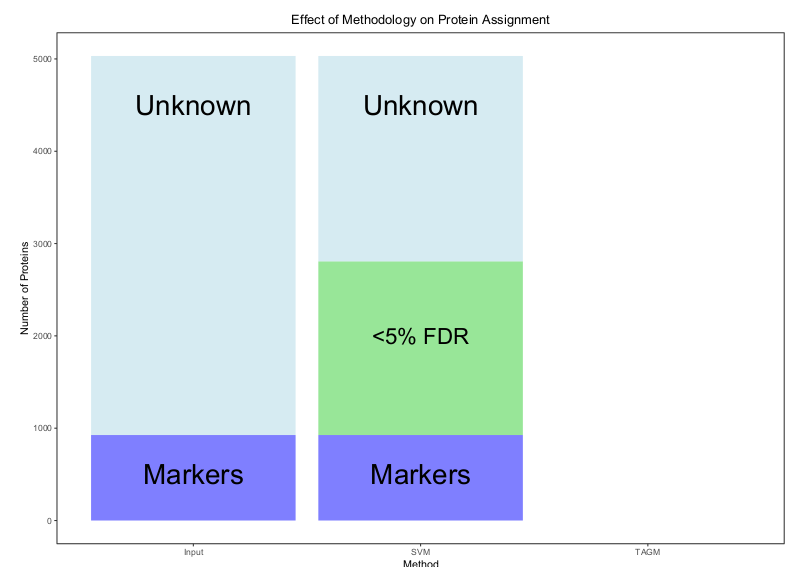
\includegraphics[width=.8\linewidth]{./figs_all/preConcludePlot.png}
  \end{figure}
\end{frame}

\begin{frame}{}
    \begin{figure}[h]
    \centering
    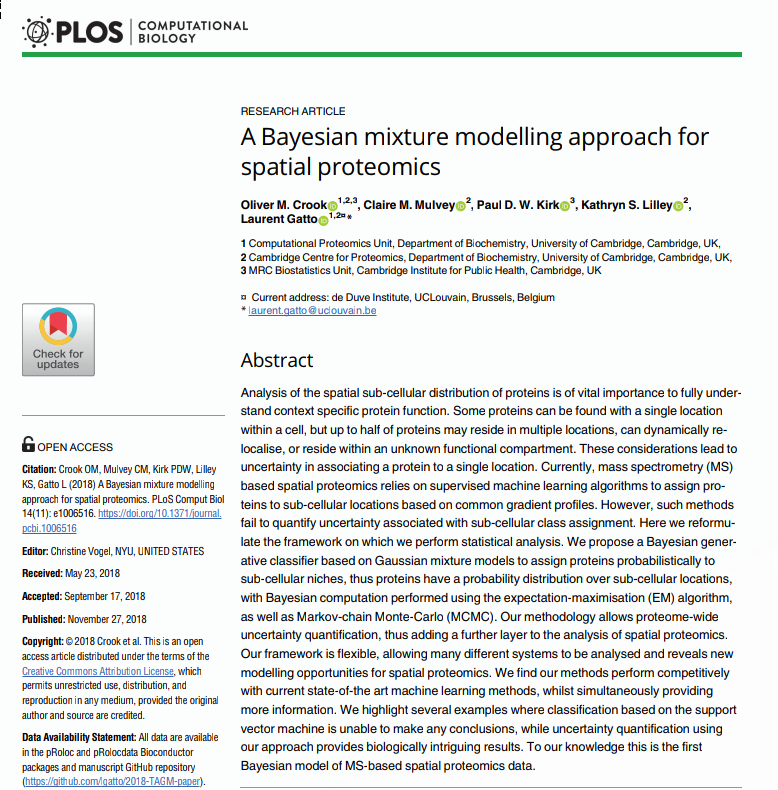
\includegraphics[width=.49\linewidth]{./figs_more/plostagm.png}
    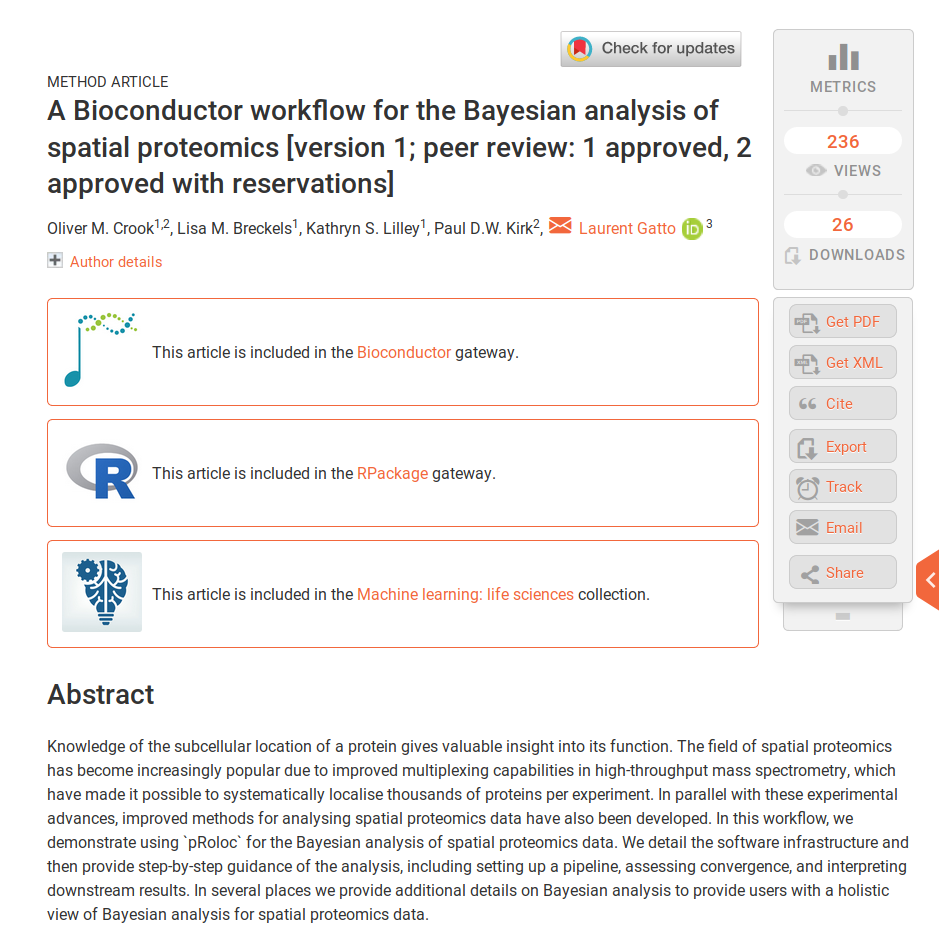
\includegraphics[width=.49\linewidth]{./figs_more/f1000tagm.png}
    \caption{See \cite{Crook:2018} and \cite{Crook:2019}.}
  \end{figure}    
\end{frame}


\begin{frame}{A Bayesian Mixture Modelling Approach For Spatial Proteomics}

  \begin{itemize}

    \item<+-> \textit{T Augmented Gaussian Mixture model (TAGM)} is a
      \textbf{multivariate Gaussian generative model} for MS-based
      spatial proteomics data. It posits that each annotated
      sub-cellular niche can be modelled by a multivariate Gaussian
      distribution.

    \item<+-> With the prior knowledge that many proteins are not
      captured by known sub-cellular niches, we augment our model with
      an \textbf{outlier component}. Outliers are often dispersed and
      thus this additional component is described by a heavy-tailed
      distribution: the multivariate Student's t-distribution, leading
      us to a \textit{T Augmented Gaussian Mixture model}.

    \item<+-> This methodology allows proteome-wide
      \textbf{uncertainty quantification}, thus adding a further layer
      to the analysis of spatial proteomics.

  \end{itemize}
\end{frame}


\begin{frame}{}

    We initially model the distribution of profiles associated with
    proteins that localise to the $k$-th component as multivariate
    normal with mean vector $\boldsymbol{\mu}_k$ and covariance matrix
    $\Sigma_k$, so that:

    \begin{align}
      {\bf x}_i | z_i = k \quad \sim \mathcal{N}(\boldsymbol{\mu}_k, \Sigma_k) \label{equation::preq}
    \end{align}

    \pause

    We extend it by introducing an additional \textit{outlier
      component}. To do this, we augment our model by introducing a
    further indicator latent variable $\phi$. Each protein ${\bf x}_i$
    is now described by an additional variable $\phi_i$, with $\phi_i
    = 1$ indicating that protein ${\bf x}_i$ belongs to a organelle
    derived component and $\phi_i = 0$ indicating that protein ${\bf
      x}_i$ is not well described by these known components. This
    outlier component is modelled as a multivariate T distribution
    with degrees of freedom $\kappa$, mean vector $\bf{M}$, and scale
    matrix $V$.

    \begin{align}
      {\bf x}_i | z_i = k, \phi_i \quad \sim \mathcal{N}(\boldsymbol{\mu}_k, \Sigma_k)^{\phi_i}\mathcal{T}(\kappa, \boldsymbol{M}, V)^{1 - \phi_i }
    \end{align}


\end{frame}


\begin{frame}[fragile]{}
      \begin{figure}
        \sidebysidecaption{0.65\linewidth}{0.3\linewidth}{
          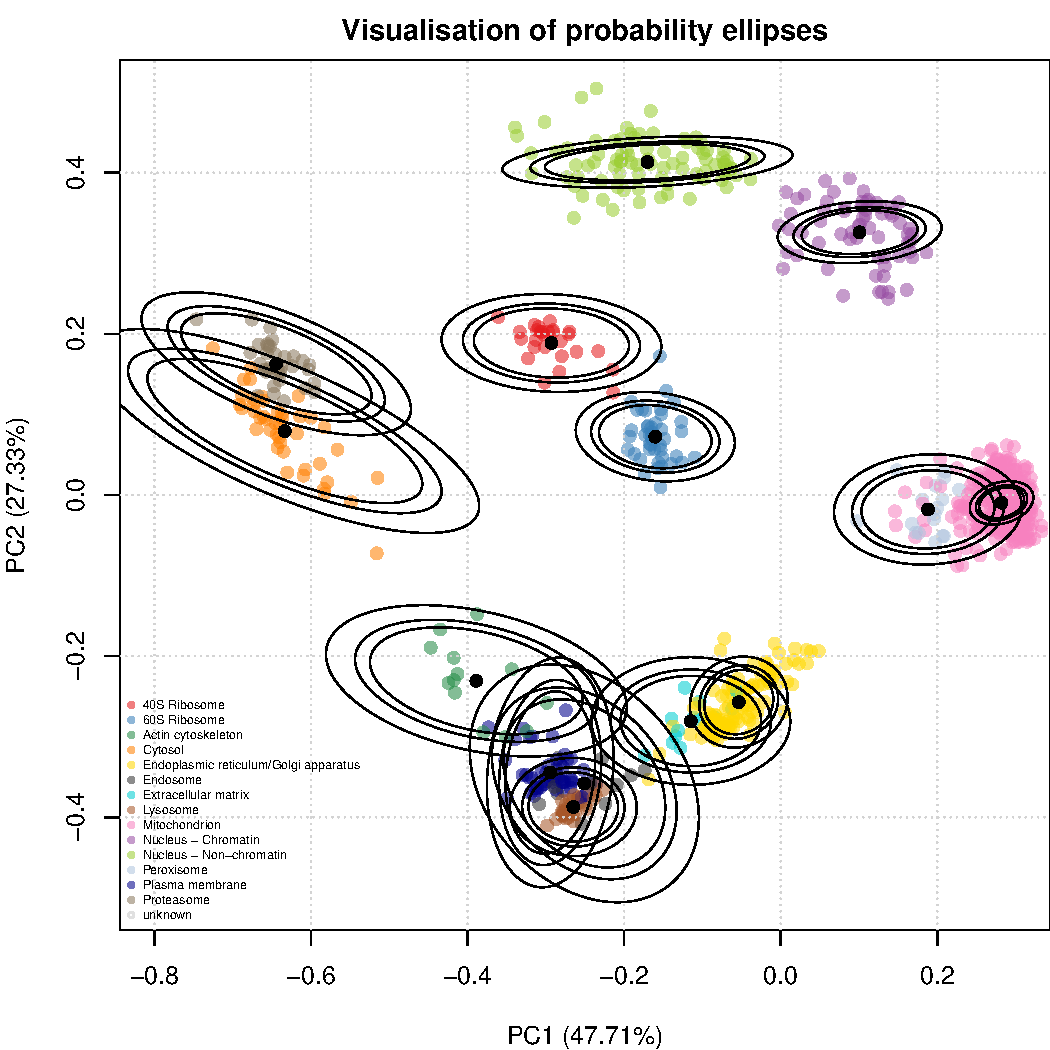
\includegraphics[width=1\linewidth]{./figs_all/pca12-ellipses-1.pdf}
        }{
          \caption{\scriptsize \justifying Illustration of how the
            TAGM model describes the pluripotent mouse embryonic stem
            cell data. Each ellipse contains a proportion of total
            probability of a particular multivariate Gaussian density.
            The outer ellipse contains $99\%$ of the total probability
            whilst the middle and inner ellipses contain $95\%$ and
            $90\%$ of the probability respectively.}
          \label{fig:tagm}
        }
      \end{figure}

      %% NOTE that while some sub-cellular clusters overlap along PC1 and
      %% PC2, they are separated along additional dimensions.

\end{frame}

\begin{frame}{}
      \begin{figure}
        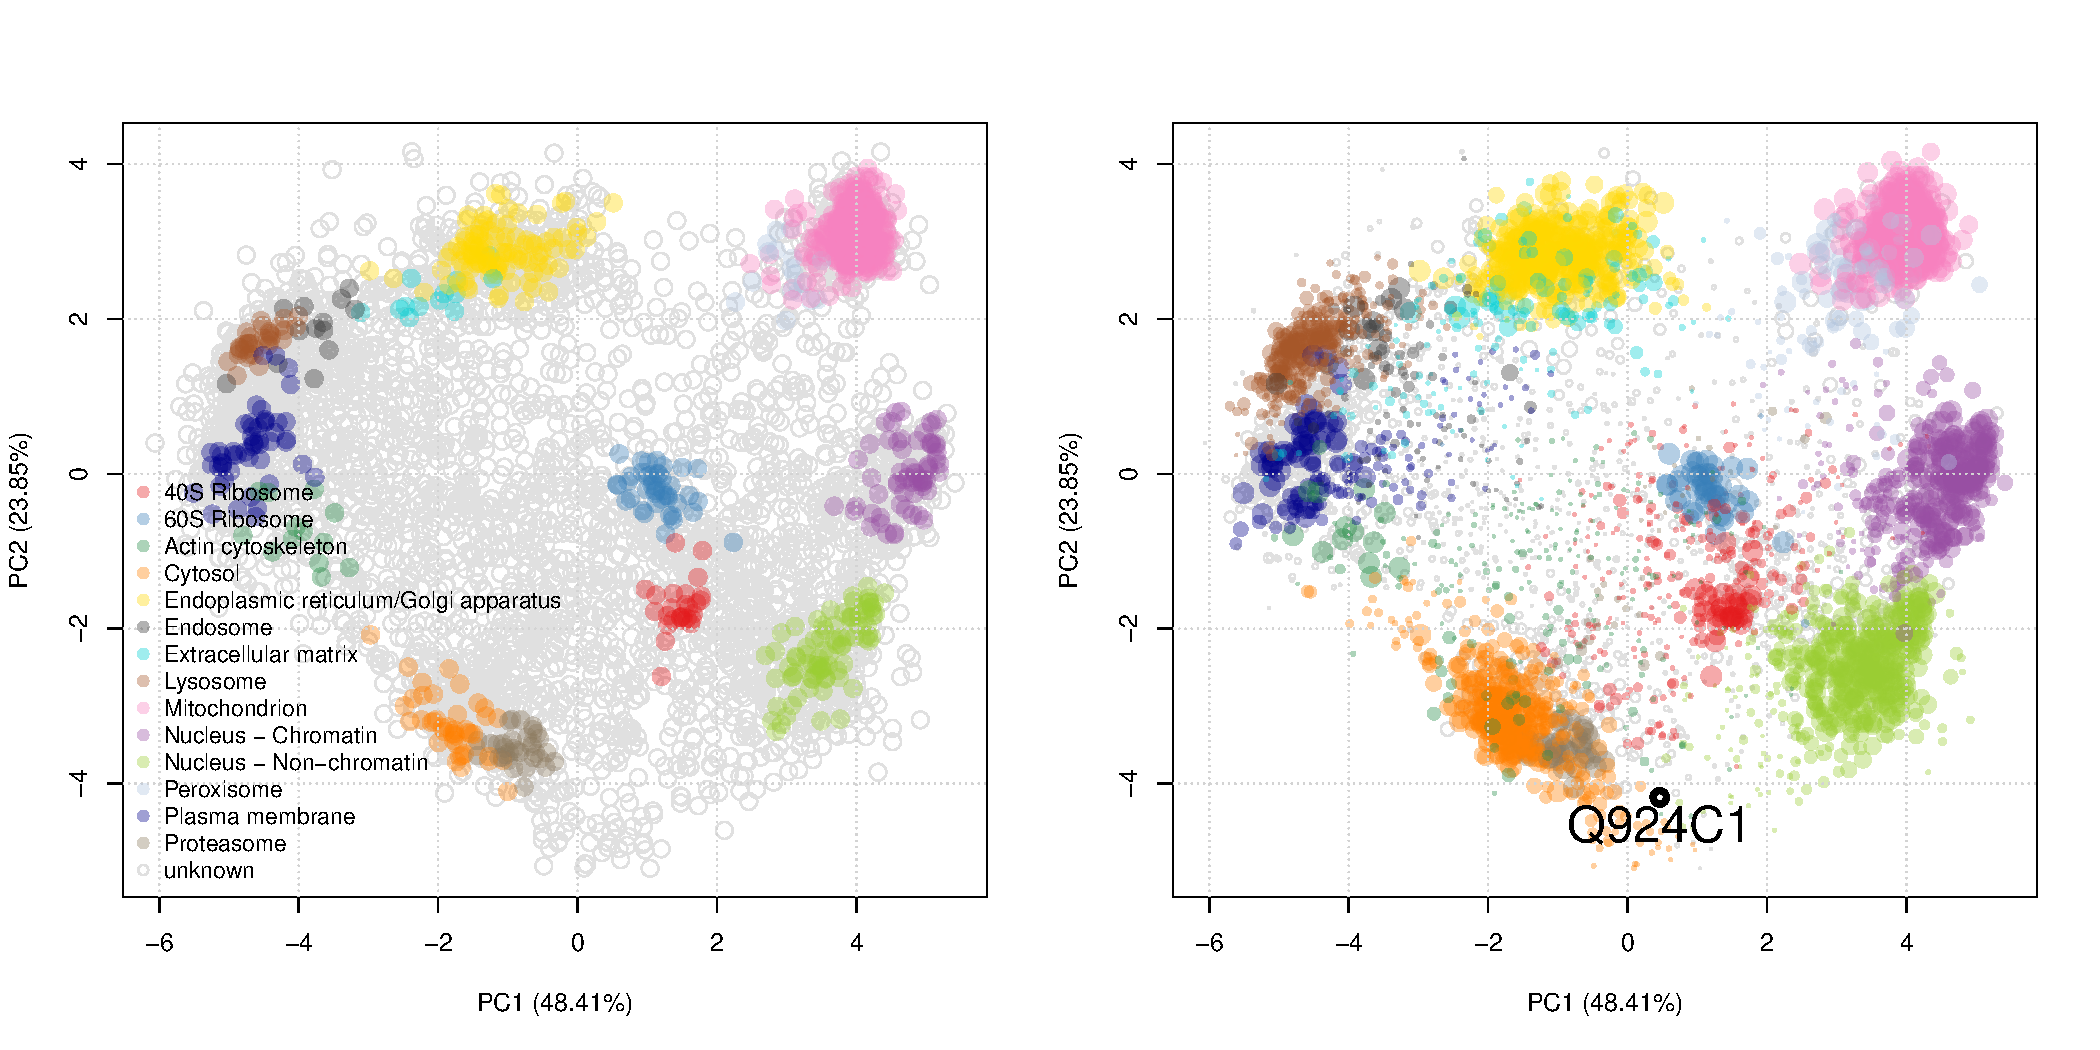
\includegraphics[width=1\linewidth]{./figs_all/tagm_pca_res.pdf}
        \caption{Assignment of proteins of
          \textit{unknown} location to one of the annotated
          classes. The dots are scaled according to the protein
          assignment probabilities.}
      \end{figure}
\end{frame}

\begin{frame}{}
  \begin{figure}
    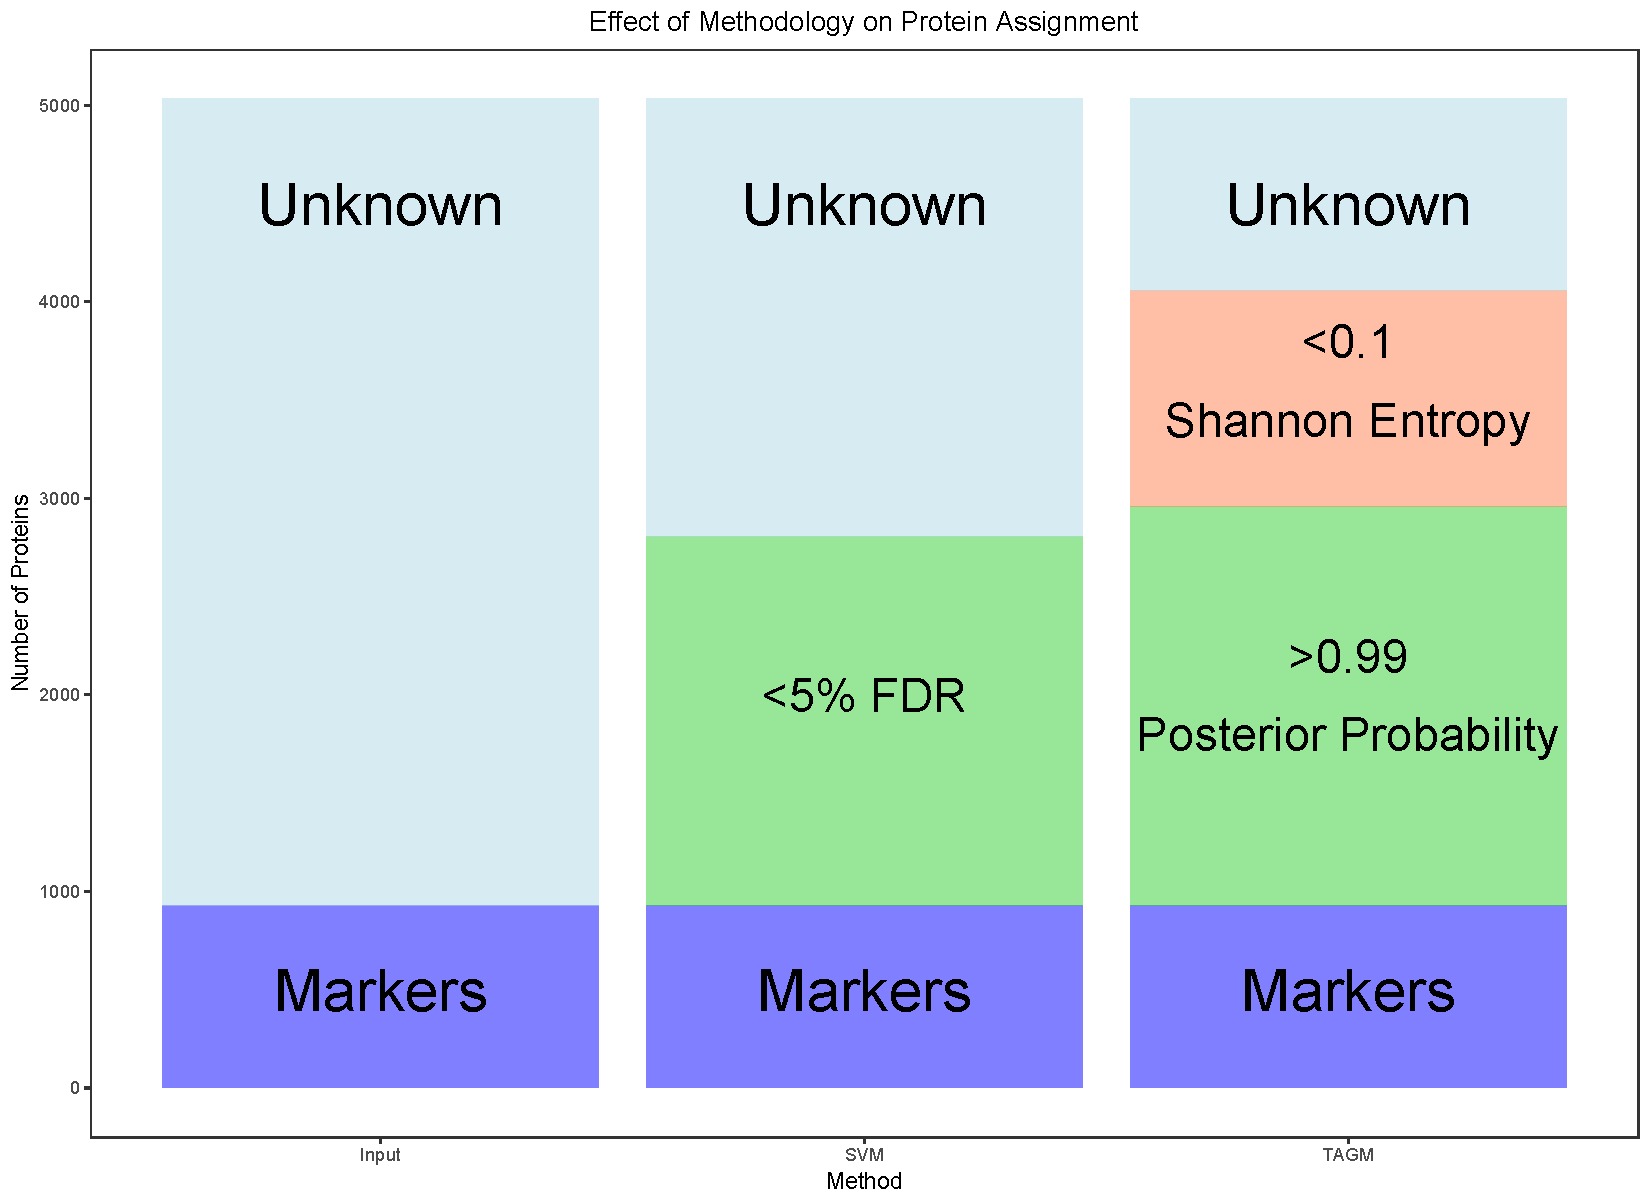
\includegraphics[width=.8\linewidth]{./figs_all/ConcludePlot.pdf}
  \end{figure}
\end{frame}

\begin{frame}
  \begin{figure}
    \centering
    \sidebysidecaption{0.55\linewidth}{0.42\linewidth}{
      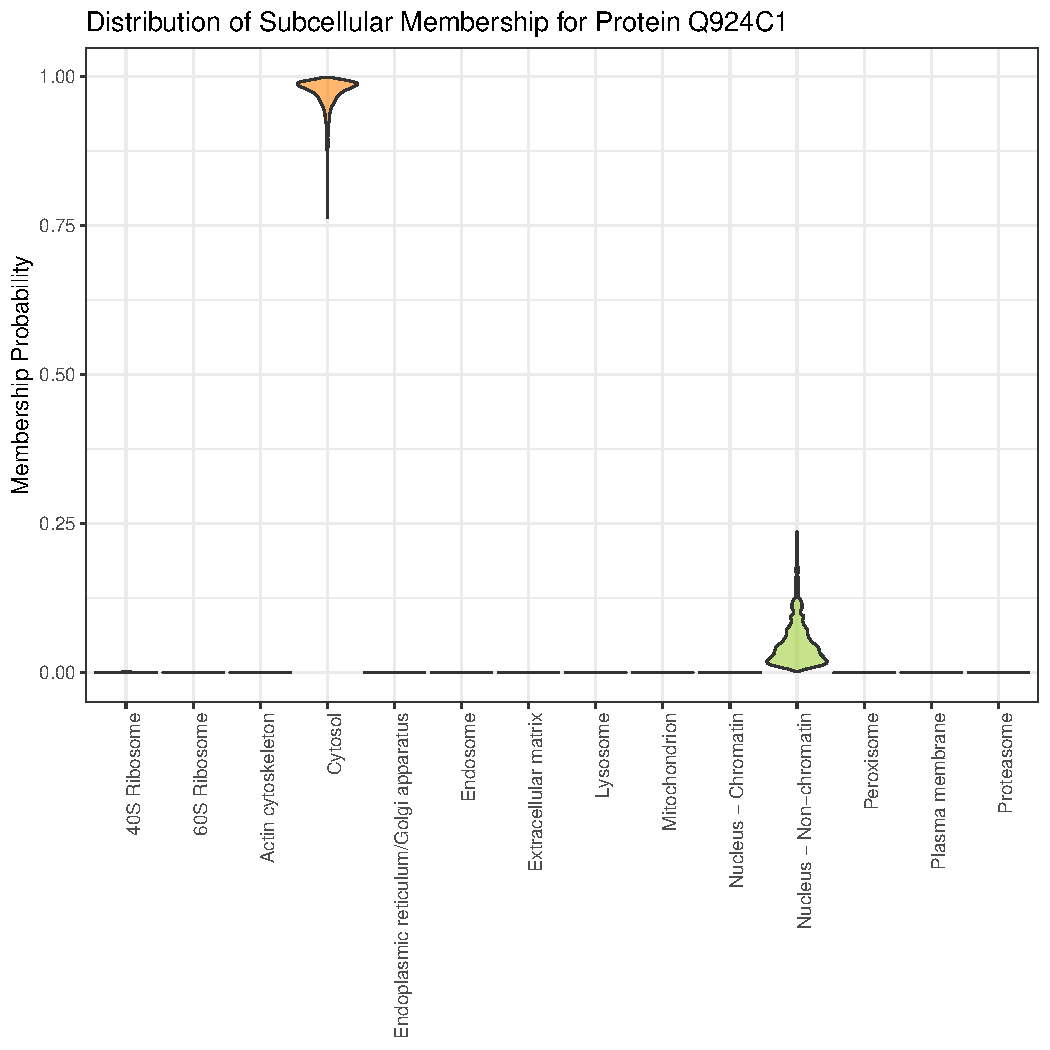
\includegraphics[width=1\linewidth]{./figs_all/Q924C1-prob-1.pdf}
    }{
    \caption{\scriptsize \justifying Exportin 5 (Q924C1) forms part of
      the micro-RNA export machinery, transporting miRNA from the
      nucleus to the cytoplasm for further processing.  It then
      translocates back through the nuclear pore complex to return to
      the nucleus to mediate further transport between nucleus and
      cytoplasm. The model correctly infers that it most likely
      localises to the cytosol but there is some uncertainty with this
      assignment. This uncertainty is reflected in possible assignment
      of Exportin 5 to the nucleus non-chromatin and reflects the
      multi-location of the protein.}  }
    %% NOTE SVM failed to classify exportin 5 to any of the two
    %% biologically plausible locations, arguably due to the similarity
    %% of the cytosol and peroxysome, to which it got assigned.

  \end{figure}
\end{frame}


\begin{frame}{Whole sub-cellular proteome uncertainty}
  \begin{figure}
    \centering
    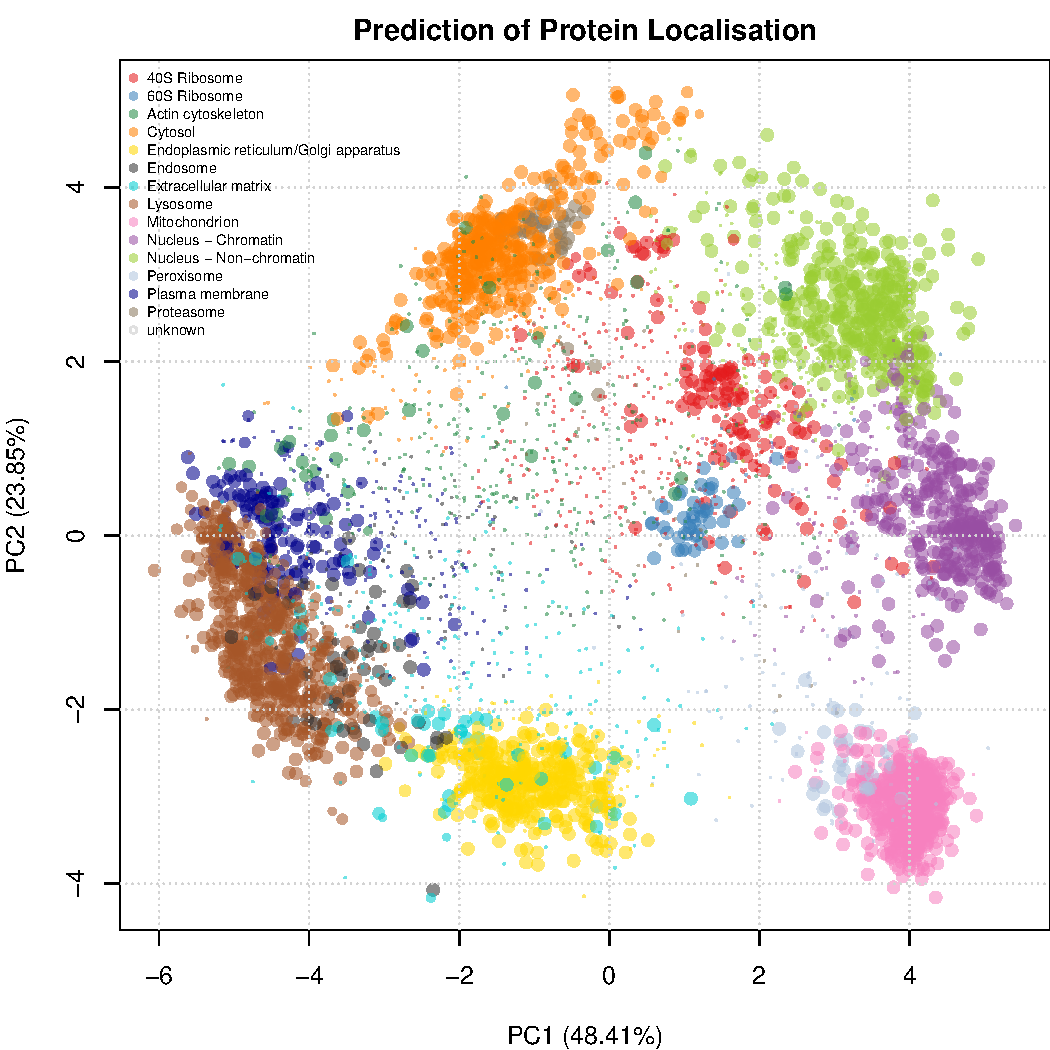
\includegraphics[width=.32\linewidth]{./figs_all/pca-tagm-mcmc-1.pdf}
    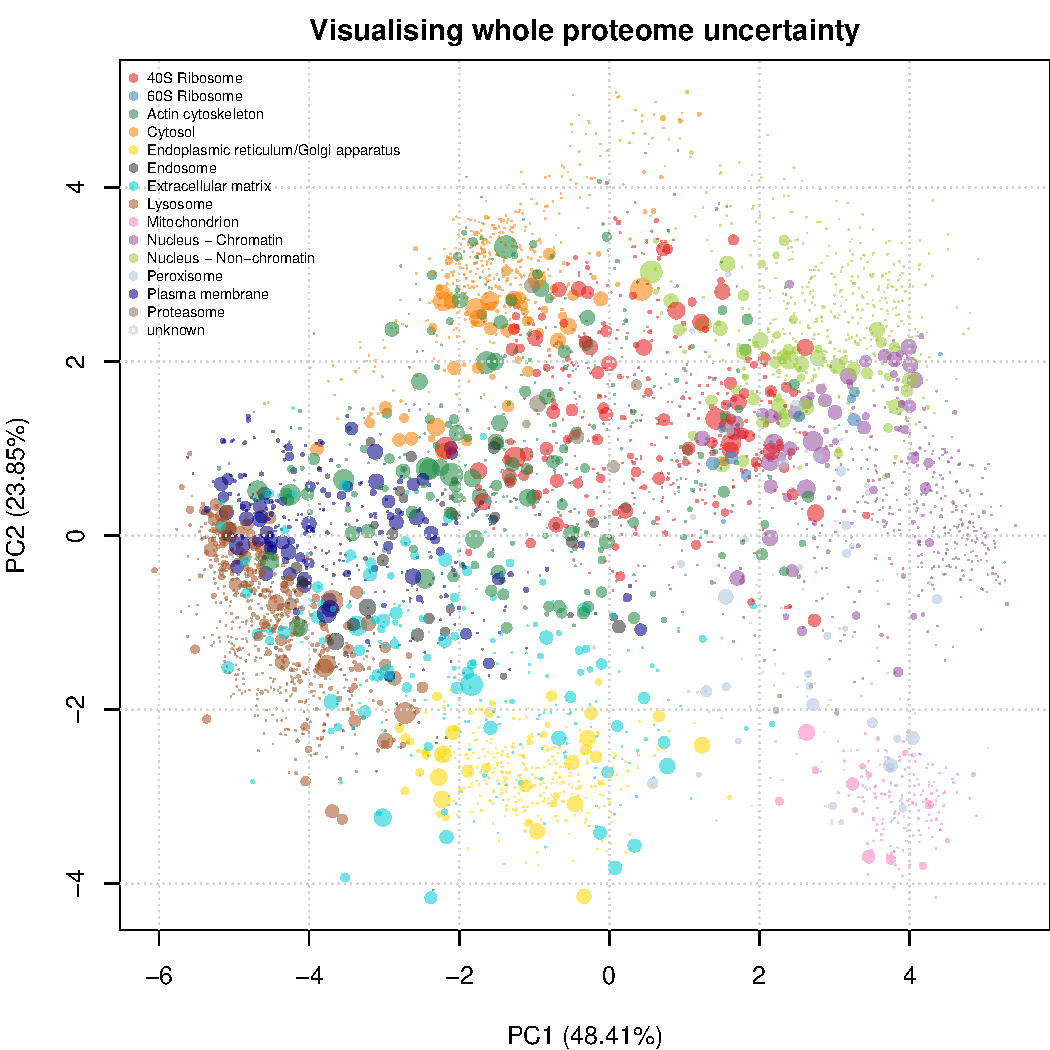
\includegraphics[width=.32\linewidth]{./figs_all/pca-tagm-map-1.pdf}
    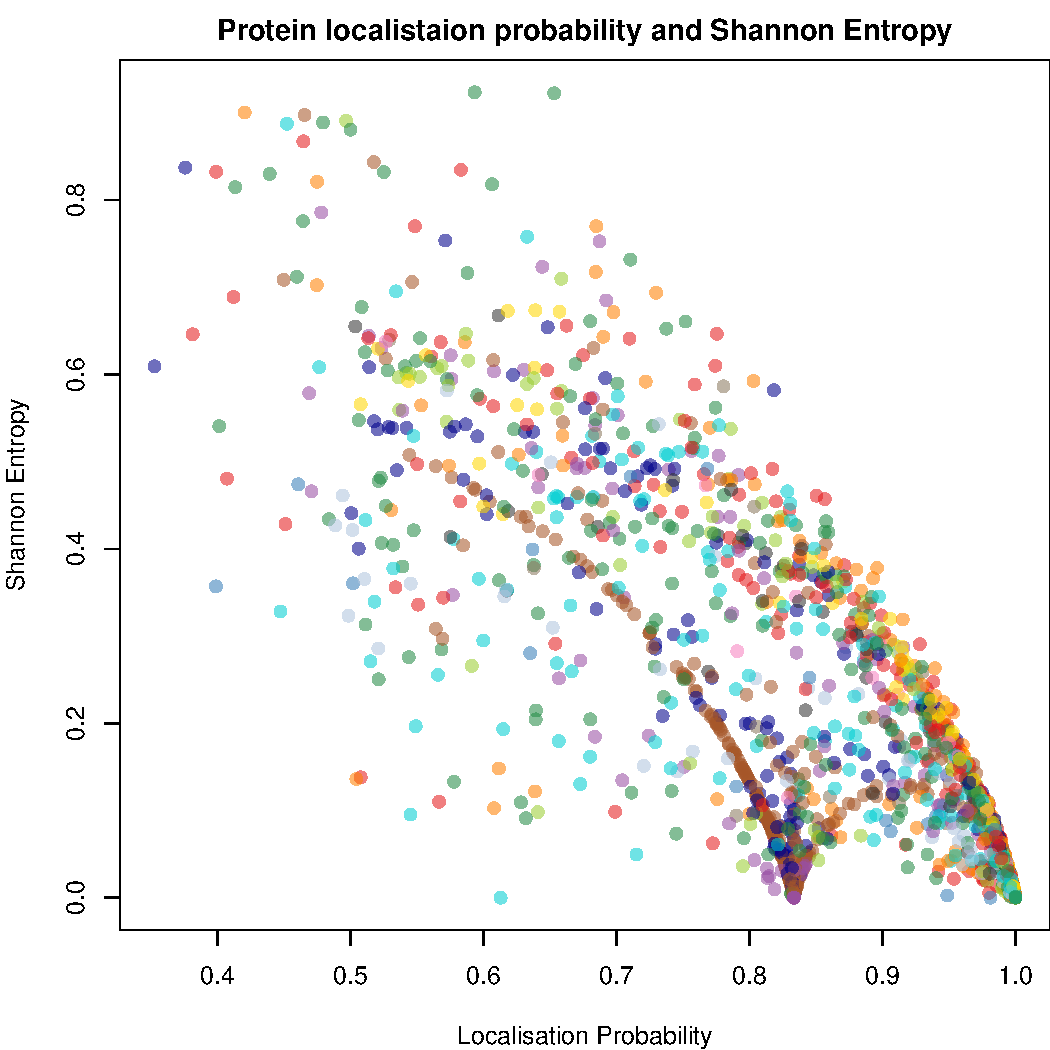
\includegraphics[width=.32\linewidth]{./figs_all/prob-vs-shannon-1.pdf}
  \end{figure}
\end{frame}

